\let\negmedspace\undefined
\let\negthickspace\undefined
%\RequirePackage{amsmath}
\documentclass[journal,12pt,twocolumn]{IEEEtran}
 \usepackage[utf8]{inputenc}
 \usepackage{graphicx}
 \usepackage{amsmath}
 \usepackage{amsfonts}
 \usepackage{amssymb}
 \usepackage{enumitem}
\usepackage{mathtools}
\usepackage[breaklinks=false]{hyperref}
\usepackage{listings}
\usepackage{calc}

\newcommand{\BEQA}{\begin{eqnarray}}
\newcommand{\EEQA}{\end{eqnarray}}
\newcommand{\define}{\stackrel{\triangle}{=}}
\bibliographystyle{IEEEtran}
%\bibliographystyle{ieeetr}

\let\vec\mathbf

\providecommand{\abs}[1]{\left\vert#1\right\vert}
\providecommand{\res}[1]{\Res\displaylimits_{#1}}
\newcommand{\myvec}[1]{\ensuremath{\begin{pmatrix}#1\end{pmatrix}}}
\newcommand{\mydet}[1]{\ensuremath{\begin{vmatrix}#1\end{vmatrix}}}

\newcommand{\question}{\noindent \textbf{Question: }}
\newcommand{\solution}{\noindent \textbf{Solution: }}


\title{Assignment 2}
\author{Vishal Vijay Devadiga (CS21BTECH11061)}
\date{}
\begin{document}
% make the title area
\maketitle
\question
\begin{enumerate}[label=]
	\item If the matrix $\myvec{6 & -x^2 \\ 2x - 15 & 10}$ is symmetric, then find the value of x.
\end{enumerate}
\solution
\begin{enumerate}[label=]
	\item For a symmetric matrix, $\vec{A}^{\top} = \vec{A}$. \\
	This implies, $a_{ij} = a_{ji}$ for all i,j. \\
	Thus, for the matrix $\vec{A}$,
	\begin{align}
		a_{12} &= a_{21}
		\\
		2x - 15 &= -x^2
		\\
		x^2 + 2x - 15 &= 0
		\\
		x^2 + 5x - 3x -15 &= 0
		\\
		x(x+5) - 3(x+5) &=0
		\\
		(x-3)(x+5) &= 0
	\end{align}
%	\begin{figure}[h]
%	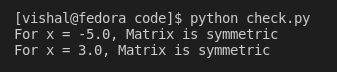
\includegraphics[width=\columnwidth]{./figs/Output.png}
%	\caption{Output of the python program}
%	\end{figure}
	The roots of the equation $x^2 + 2x -15 = 0$ are -5 and 3. \\
	Thus, the values of x for which the matrix $\myvec{6 & -x^2 \\ 2x - 15 & 10}$ is symmetric, is -5 and 3.
	
\end{enumerate}
\end{document}
